\section[Měření reaktivity]{Metody měření reaktivity a stanovení charakteristiky absorpční tyče}

\subsection{Reaktivita}

Reaktivita je jedním ze základních provozních parametrů, který ovlivňuje chování jaderného reaktoru. Její časové změny a absolutní velikost mají bezprostřední vliv na bezpečný provoz reaktoru a jsou proto limitovány. S reaktivitou je svázána řada provozních parametrů reaktoru, jejichž detailní znalost je nezbytná pro jeho provoz. Patří k nim (resp. je posuzováno pro VR-1):

\begin{itemize}%[noitemsep]
    \item podkritičnost odstaveného reaktoru,
    \item maximální přebytek reaktivity (MPR) -- zásoba kladné reaktivity, vázaná při kritickém stavu reaktoru řídicími tyčemi E1, E2, R1 a~R2,
    \item provozní přebytek reaktivity (PPR) -- zásoba kladné reaktivity, vázaná při kritickém stavu reaktoru řídicími tyčemi R1 a~R2,
    \item Maximální rychlost uvolnění kladné reaktivity při pohybu tyče určovaná vztahem (vychází z poruchové teorie): 
    \begin{equation} \label{eq:rychlost_reak-vyp}
v_\rho \leq {{2 \cdot \rho_T \cdot v_T} \over {H}}
\end{equation}

\noindent kde:

$
\begin{array} {ll}
\rho_T &  \text{váha tyče } T \\
v_T &  \text{rychlost pohybu tyče } T \\
H & \text{horní koncová poloha tyče (680 mm)} \\
\end{array}
$
    \item kompenzační schopnost reaktoru -- zásoba záporné reaktivity, vázaná při kritickém stavu reaktoru všemi absorpčními tyčemi.
    \item účinnost bezpečnostních ochran: \begin{equation} \label{eq:UBO}
\frac{\sum\limits_{i=1}^{7}\rho_i - \rho_{max}}{MPR}
\end{equation}
$
\begin{array} {ll}
\rho_i &  \text{kompenzační schopnost i-té absorpční tyče} \\
\rho_{max} & \text{kompenzační schopnost absorpční tyče s~maximálním účinkem} \\
\end{array}
$
\end{itemize}
V Tabulce \ref{tab:VýsledkyzKEX} jsou uvedeny vypočtené parametry pro AZ C12-C (zóna reaktoru VR-1). 

\begin{table}[!hb]
  \centering
  \caption{Výpočtem určené základní provozní hodnoty AZ}
  \begin{tabular}{c c c}
    \toprule
     hodnocený parametr & zjištěná hodnota & limitní hodnota\\
    \midrule
    % MPR & 2,38 $\pm$ 0,01 $\beta_{ef}$ & není limitován\\
    MPR & 2,39 $\pm$ 0,02 $\beta_{ef}$ & není limitován\\
    PPR (E2=170 mm) & 0,59 $\pm$ 0,02 $\beta_{ef}$ & $\leq$ 0,7 $\beta_{ef}$\\
    % PPR (E2=160 mm) & 0,57 $\pm$ 0,01 $\beta_{ef}$ & $\leq$ 0,7 $\beta_{ef}$\\
    účinnost bezpečnostních ochran & 2,38 $\pm$ 0,02
    & $\geq$ 1,5\\
    podkritický stav pro odstavený reaktor & -8,53 $\pm$ 0,02 $\beta_{ef}$ & $\leq$ -3 $\beta_{ef}$\\
    max. rychlost uvolnění reaktivity při pohybu tyče & $\approx 0,05 \beta_{ef} \cdot s^{-1}$ & $\leq$ 0,1 $\beta_{ef} \cdot s^{-1}$\\
    \bottomrule
  \end{tabular}
  \label{tab:VýsledkyzKEX}
\end{table}
\newpage
Reaktivita představuje relativní odchylku reaktoru od kritického stavu, čímž je dána i její souvislost s koeficientem násobení:

\begin{equation}
    \boxed{\rho = \frac{k_{\text{ef}} - 1}{k_{\text{ef}}}.}
\end{equation}

Někdy se lze setkat také s vyjádřením ve tvaru s přirozeným logaritmem:

\begin{equation}
    \rho = \ln(k_{\text{ef}}),
\end{equation}

Platnost tohoto vztahu je však omezena pouze na hodnoty blízké kritickému stavu reaktoru. Plyne z Taylorova rozvoje přirozeného logaritmu okolo jedničky, kde $\ln{x} \approx x - 1$, ale nechápu, proč by to někdo dělal\footnote{Mám pocit, že je to pro zrychlení výpočtu a že to takhle aplikují systémy na ETE.}.

Jak vyplývá z definice reaktivity, jedná se o bezrozměrnou veličinu, nicméně z praktických důvodů se používají pomocné jednotky, respektive jejich násobky:

\begin{align*}
    \rho (\%) &= \frac{k_{\text{ef}} - 1}{k_{\text{ef}}} \cdot 100, \\
    \rho (\text{pcm}) &= \frac{k_{\text{ef}} - 1}{k_{\text{ef}}} \cdot 10^5, \\
    \rho (\beta_{\text{ef}}) &= \frac{k_{\text{ef}} - 1}{k_{\text{ef}}}\cdot \dfrac{1}{\beta_\text{ef}}.
\end{align*}

V procentech se reaktivita prakticky neuvádí, jednotky pcm se používají na energetických reaktorech a $\beta_\text{ef}$ je nejčastěji na výzkumných reaktorech, protože palivo moc nevyhořívá a hodnota $\beta_\text{ef}$ se zásadně nemění. V anglicky psané literatuře se obvykle používá místo jednotek $\beta_{\text{ef}}$ označení \$, respektive jeho setina tj. ¢.

\subsection{Metody měření reaktivity}

V podstatě se aplikují pouze pro měření podkritičnosti (až na metodu kladné periody), případně pro určování váhy regulačních orgánů (uvedu reaktor do kritického stavu, vložím absorbátor, změřím podkritičnost systému, což je právě váha vloženého absorbátoru). 

Pokud máme kritický a nadkritický stav, tak to změřím celkem jednoduše za pomoci podílu odezvy na detektoru dvěmi po sobě jdoucími měřeními (viz měření na VR-1). Problém je měření podkritičnosti, což takto nejde (na detektoru nenaměřím v podstatě nic). Existuje poměrně dost metod měření podkritičnosti, ale my jsme si tak nějak říkali jen o následujících:

\begin{itemize}%[noitemsep]
    \item Rod-Drop,
    \item Source-Jerk,
    \item Násobení zdroje,
    \item Kladná perioda,
    \item Využití reaktimetru.
%    \item Feynman alfa.
\end{itemize}

\subsubsection{Rod-Drop a Source-Jerk -- okamžitý skok}

Metoda \textbf{Rod-Drop} se používá k určování velikosti záporné reaktivity skokově vnesené do AZ kritického reaktoru, např. pádem absorpční tyče. 

Metoda \textbf{Source-Jerk} slouží k určení velikosti podkritického stavu reaktoru s vnějším zdrojem neutronů za pomoci jeho odstranění.

Výchozím stavem obou metod je reaktor v kritickém stavu (v případě Rod-Drop jde skutečně o kritický stav, v případě Source-Jerk jde o podkritický stav s vnějším zdrojem neutronů, což ho přivede do ustáleného stavu). V tomto ustáleném stavu máme konstantní hustotu neutronů $n_0 = \text{konst.} \rightarrow \frac{dn(t)}{\text{d}t} = 0$. Tento vztah dosadíme do rovnice jednobodové kinetiky:

\begin{equation*}
0 = \frac{\textcolor{red}{\rho}-\beta_{\text{ef}}}{\Lambda} \cdot n_0 + \sum_{i=1}^6 \lambda_i \cdot c_{i0} +\textcolor{red}{S}
\end{equation*}

Předpokládáme-li, že v krátkém časovém okamžiku (odpovídající střední době života okamžitých neutronů) po zavedení tyče do AZ, nebo při vypnutí zdroje neutronů, \textbf{nedojde ke změně koncentrace mateřských jader zpožděných neutronů} (prekurzorů $c_{i0}$) a taktéž bude-li dále platit $\frac{dn(t)}{\text{d}t} = 0$, pak pro kvazistatický stav s nižší hustotou neutronů $n_1$ (to je ten stav po zavedení záporné reaktivity) a $\rho < 0$ bude platit:

\begin{equation*}
0 = \frac{\rho-\beta_{\text{ef}}}{\Lambda} \cdot n_1 + \sum_{i=1}^6 \lambda_i \cdot c_{i0}.
\end{equation*}

Dosazením těchto dvou rovnic do sebe a se započtením korekce na odezvu pozadí $n_\text{B}$ dostáváme finální vztah:

\begin{equation}
    \boxed{ \dfrac{\rho}{\beta_\text{ef}}=1-\dfrac{n_0 - n_\text{B}}{n_1 -n_\text{B}}.}
\end{equation}

V reálném měření prostě $n_0$, $n_1$ a $n_\text{B}$ odpovídají četnostem na detektorech (předpokládáme, že detekční účinnost je stejná a navzájem se ve zlomku vykrátí, jde nám o poměr).

\begin{figure}[H]
    \centering
    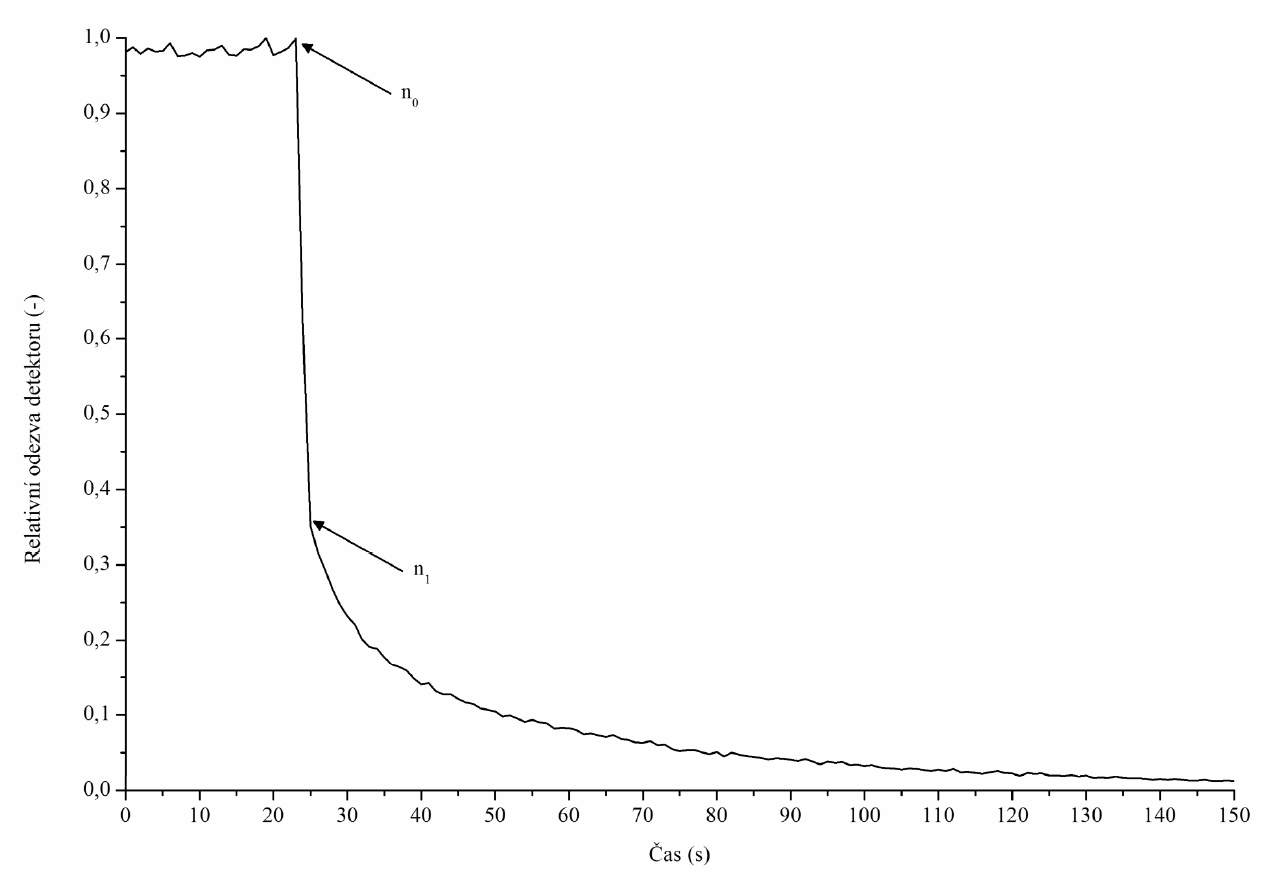
\includegraphics[scale=0.35]{img/RodDropMěření.png}
    \caption{Rod-Drop měření.}
    %\label{fig:Rod-Drop}
\end{figure}

\subsubsection{Rod-Drop a Source-Jerk -- integrálně}

Pro obě metody lze odvodit vztah pro reaktivitu i v případě \textbf{uvažování změn koncentrace mateřských jader zpožděných neutronů}, ke které dochází po vyvolání dynamické změny v reaktoru. Nalezení příslušných vztahů vychází opět z řešení rovnic jednobodové kinetiky. Integrální metoda spočívá v integraci obou rovnic od okamžiku, kdy byla vyvolána dynamická změna v reaktoru (pád absorpční tyče do AZ nebo odstranění neutronového zdroje z AZ) až po okamžik, kdy hustota zpožděných neutronů poklesne k nule:

\begin{equation*}
    \int_0^\infty d n(t)= \dfrac{\rho - \beta_{\text{ef}}}{\Lambda}\cdot \int_0^\infty n(t) \text{d}t + \sum_{i=1}^6 \lambda_i \int_0^\infty c_i(t) \text{d}t + \int_0^\infty S(t) \text{d}t 
\end{equation*}

\begin{equation*}
    \int_0^\infty dc_i(t) = \frac{\beta_{\text{ef}, i}}{\Lambda}\cdot \int_0^\infty n(t) \text{d}t - \lambda_i \int_0^\infty c_i(t) \text{d}t
\end{equation*}

Abychom mohli vyřešit tyto rovnice, je nutné aplikovat úpravy integrálů a zároveň určit podmínky:
\begin{equation*}
\int_0^\infty dn(t) = n(\infty) - n(0) \quad \text{a} \quad \int_0^\infty dc_i(t) = c_i(\infty) - c_i(0) 
\end{equation*}

a podmínky:

\begin{equation*}
n(t=0) = n_0 \quad \text{a} \quad c_i(t=0) = c_{i0} \hspace{2cm} n(t \to \infty) \to 0 \quad \text{a} \quad c_i(t \to \infty) \to 0 
\end{equation*}

Přesné odvození je ve skriptech, ale finální rovnice vede na tvar:

\begin{equation}
\boxed{ \frac{\rho}{\beta_{\text{ef}}} = -\frac{n_0 \left( \sum_{i=1}^6 \frac{\beta_{\text{ef},i}}{\beta_{\text{ef}} \lambda_i} \right)}{\int_0^\infty n(t) \text{d}t} \approx -\frac{(n_0-n_\text{B}) \cdot A}{\int_0^{300\text{ s}} \left( n(t)-n_\text{B}\right) \text{d}t}.}
\end{equation}

Konstanta $A$ je charakteristická pro každou AZ dle geometrie a vsázky. Počítá se numericky (např. Serpentem) a pohybuje se řádově mezi 12-15 $\beta_\text{ef}\cdot s$. Zároveň se musí opět odečíst korekce na pozadí $n_\text{B}$ a integrovat stačí do doby, než vymřou všechny prekurzory zpožděných neutronů (my na VR-1 jsme většinou čekali 300 s). Při měření je nejsložitější určit počátek integrálu, protože tyč/zdroj nějakou dobu padá/odstřeluje se, ale rovnice předpokládají okamžité zasunutí/odstřelení. To samé detektory snímají pouze v předem definovaných časových krocích a může se stát, že tento krok dostatečně nepostihne okamžik zavedení záporné reaktivity.

\begin{figure}[H]
    \centering
    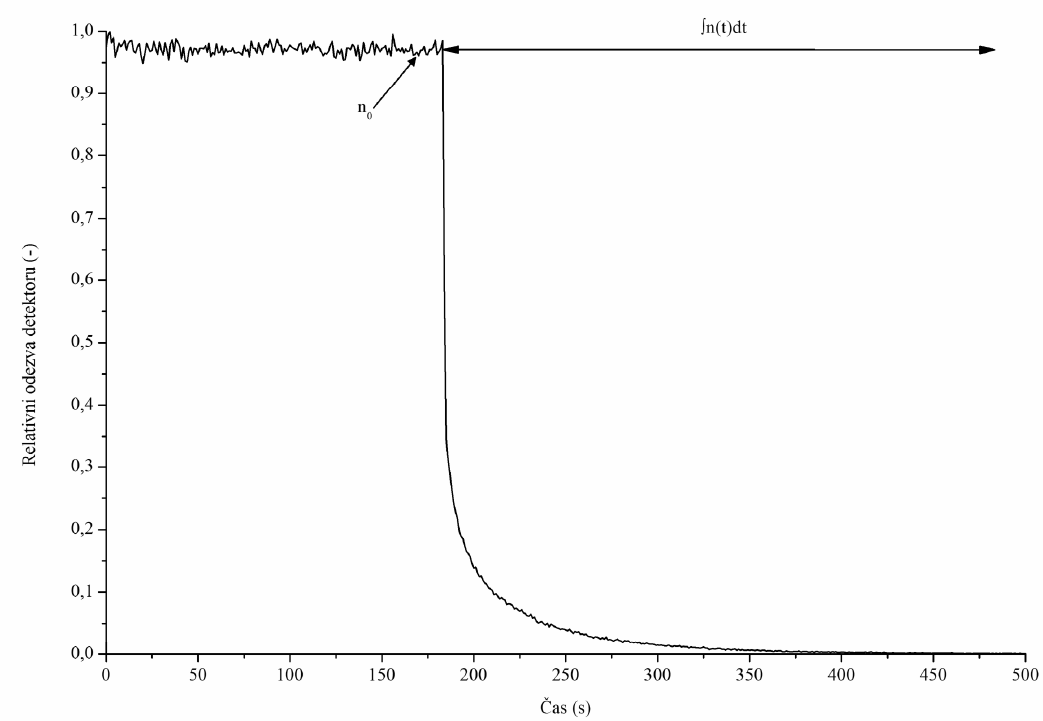
\includegraphics[scale=0.3]{img/RodDrop.png}
    \caption{Rod-Drop měření.}
    \label{fig:Rod-Drop}
\end{figure}

\subsubsection{Násobení zdroje}

Další metoda, která se využívá k určování podkritického stavu reaktoru, je metoda násobení zdroje. \textbf{Tato metoda se používá jako on-line metoda na měření reaktivity v jaderných reaktorech.}

Metoda vychází z kombinace dvou měření:
\begin{itemize}
    \item reaktor v podkritickém stavu se zdrojem.
    \item reaktor v kritickém stavu se zdrojem.    
\end{itemize}
Vychází se opět z rovnic bodové kinetiky (odvození ve skriptech). Máme podkritický systém (ten co měřím) se zapnutým neutronovým zdrojem. Tím se nám reaktor ustálí, díky čemuž můžeme stanovit zdrojový člen $n_0$. V dalším kroku přivedeme reaktor do kritického stavu (zdroj je furt zapnutý), což má za následek \textbf{lineární nárůst četnosti}. V tomto okamžiku změříme směrnici $k$ tohoto nárůstu (viz Obrázek \ref{fig:NásobeníZdroje}) a jednoduchým dosazením hodnot $n_0$ a směrnice $k$ do rovnice~\eqref{eq:NZ}. 

Z rovnic bodové kinetiky, získáme nehomogenní
diferenciální rovnici druhého řádu s konstantními koeficienty a řešení vede na tvar

\begin{equation*}
n(t) = \tilde{n}(t) + \hat{n}(t) = K_1 + K_2 \cdot e^{-\left(\frac{\beta_{\text{eff}}}{\ell} + \lambda\right)t} + \frac{S \cdot \ell}{\ell} \cdot t,
\end{equation*}
člen s exponenciálním poklesem lze zanedbat a poté rovnice přechází na tvar:
\begin{equation} \label{eq:NZ}
    \boxed{ \rho (\beta_\text{ef}) = -\frac{\overline{\ell}\cdot k}{(n_\text{0} - n_\text{B}) \cdot \beta_\text{ef}}, }
\end{equation}

kde $\overline{\ell}$ značí střední dobu života jedné generace neutronů, $\beta_\text{ef}$  značí efektivní podíl zpožděných neutronů (obě dvě jsou konstanty) a $k$ značí směrnici nárůstu kritického systému se zdrojem. V tento moment totiž platí:

\begin{equation*}
 n(t) = \frac{S \cdot \ell}{\bar{\ell}} t + \text{konst.} = k\cdot t + \text{konst.}
\end{equation*}

\begin{figure}[H]
    \centering
    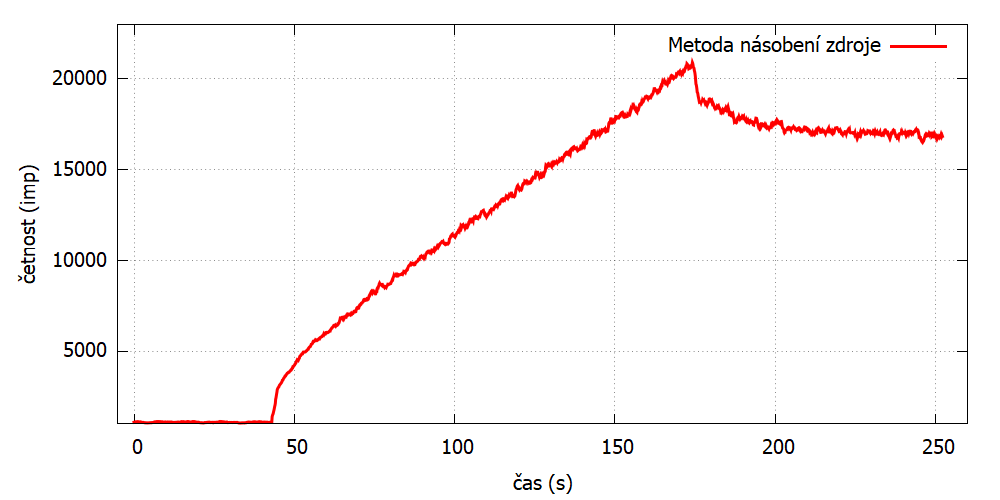
\includegraphics[scale=0.4]{img/NásobeníZdroje.png}
    \caption{Násobení zdroje.}
    \label{fig:NásobeníZdroje}
\end{figure}

\subsubsection{Kladná perioda}

Metoda kladné periody se používá k určování velikosti kladné reaktivity, která byla "skokově" vnesena do reaktoru v kritickém stavu. Tato reaktivita je pak určována na základě měření periody reaktoru v nadkritickém stavu.

Vztah mezi reaktivitou a periodou můžeme nalézt opět na základě řešení rovnic jednobodové kinetiky. Předpokládejme, že reaktor je na počátku v kritickém stavu a v časovém okamžiku $ t = 0 $ je do AZ reaktoru vnesena konstantní kladná reaktivita $ \rho $. Pak můžeme aplikací Laplaceovy transformace na rovnice jednobodové kinetiky (viz otázky FJR, kapitola 8) získat následující vztah:

\begin{equation}
\boxed{ \rho = s \cdot \left( \Lambda + \sum_{i=1}^6 \frac{\beta_{\text{ef},i}}{s + \lambda_i} \right).}
\end{equation}

Řešení rovnice je graficky znázorněno na Obrázku \ref{fig:KladnáPeriodaKořeny}. Kořeny rovnice $ s $ jsou body, ve kterých vynesené křivky protínají horizontální přímku odpovídající reaktivitě $ \rho $. Z obrázku vyplývá, že v případě $ \rho > 0 $ je všech šest kořenů $ s_0, \ldots, s_6 $ záporných a pouze kořen $ s_0 $ je kladný. Je-li $ \rho < 0 $, pak je všech sedm kořenů $ s_0, \ldots, s_6 $ záporných.

\begin{figure}[H]
    \centering
    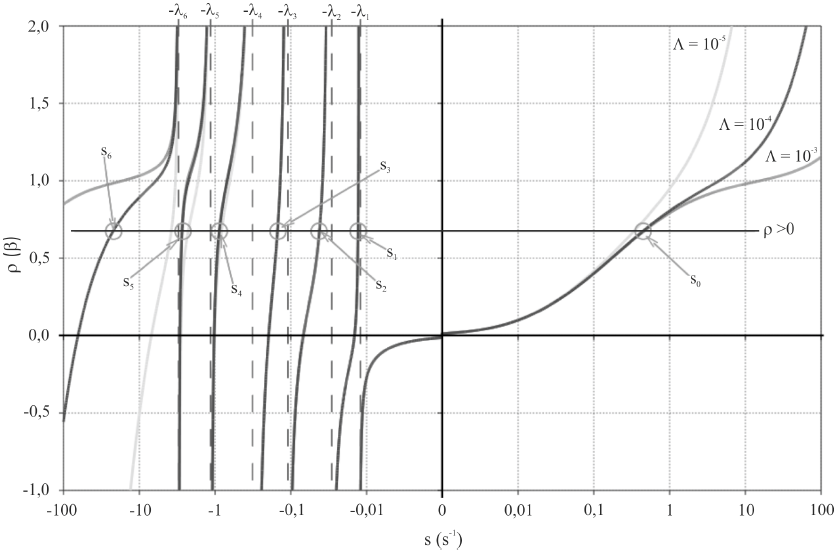
\includegraphics[scale=0.7]{img/KladnáPeriodaKořeny.png}
    \caption{Kladná perioda.}
    \label{fig:KladnáPeriodaKořeny}
\end{figure}

\subsubsection{Využití reaktimetru}

Jedním z nejčastěji používaných zařízení k měření reaktivity je tzv. reaktimetr. Jedná se o systém, který obsahuje detektor neutronů, vhodnou aparaturu (elektronické moduly) pro zpracování signálů z detektoru a procesor (počítač) s numerickým algoritmem, který na základě těchto signálů určuje reaktivitu v reálném čase.

Konečný vztah vyjadřující časovou závislost reaktivity:

\begin{equation}
    \boxed{
  \begin{multlined}
    \rho(t) = \left( \frac{\Lambda \cdot \frac{dn(t)}{\text{d}t} + \beta_{\text{ef}} - n_0 \cdot \sum_{i=1}^6 \beta_{\text{ef}, i} \cdot e^{-\lambda_i t}}{n(t)} \right) -\\
    - \left( \frac{\sum_{i=1}^6 \beta_{\text{ef}, i} \cdot \lambda_i \cdot \int_0^t n(u) \cdot e^{-\lambda_i u} \, du - \Lambda \cdot S(t)}{n(t)} \right).
\end{multlined}}
\end{equation}

Funkce $ S(t) $ popisuje vnější zdroj neutronů. Pokud je tento zdroj mimo AZ reaktoru, je $ S(t) = 0 $, jinak je $ S(t) = S_0 $ (konstanta). Hodnota $ S_0 $ závisí na konfiguraci AZ a poloze detektoru. Lze ji určit experimentálně například metodou násobení zdroje. Kalibraci reaktimetru můžeme provést také srovnáním se známou reaktivitou, kterou určíme jinou metodou.

\begin{comment}
\subsubsection{Feynman alfa}
Cílem experimentu je studium fluktuace měřené četnosti impulsů v podkritickém reaktoru s vnějším neutronovým zdrojem při použití metody Feynman-alfa (Variance-to-Mean method). Fluktuace a její změna je charakterizována rozptylem měřené četnosti, přičemž se stanovují dvě hodnoty, a to střední hodnota měřené četnosti $\bar{\text{N}}$ a rozptyl hodnoty ${\sigma_{\text{N}}}^2$. 

Feynmanova-alfa metoda je založena na šumové analýze, při které se pro různé časové okna sběru dat  na detektoru (tzv. gate-wi\text{d}th) studuje odchylka od Poissonova rozdělení získaných hodnot.
Tuto odchylku charakterizuje funkce $Y$: 

\begin{equation}
    Y = \dfrac{\sigma_\text{N}^2}{\bar{\text{N}}} -1 
    \label{eq:Y_sigma_N}
\end{equation}

Z teorie jednobodové kinetiky lze pro funkci $Y$ odvodit následující závislost:
\begin{equation}
    Y(t) = \dfrac{\bar{\varepsilon}\bar{\nu}(\bar{\nu}-1)}{\alpha^2\tau_f^2}\left(1-\dfrac{1-e^{-\alpha t}}{\alpha t} \right),
    \label{eq:Y}
\end{equation}
kde $\bar{\nu}$ je průměrný výtěžek neutronů ze štěpení, $\bar{\varepsilon}$ je značí detekční účinnost detektoru, $\tau_\text{f}$ střední doba života neutronů a rozpadová konstanta $\alpha$ je zjišťovaný parametr, charakterizující okamžité neutrony. Pro konstantu $\alpha$ platí \ref{eq:alpha_rho}:


\begin{equation}
    \alpha = \dfrac{1-k(1-\beta)}{\ell} = \dfrac{\beta-\rho}{\Lambda}.
    \label{eq:alpha_rho}
\end{equation}

Cílem měření je proložit experimentální data funkcí \ref{eq:Y} a získat hodnotu $\alpha$. Z rovnice \ref{eq:alpha_rho} lze pak při znalosti $\Lambda$ a $\beta$ určit reaktivitu systému. 

\begin{figure}[H]
    \centering
    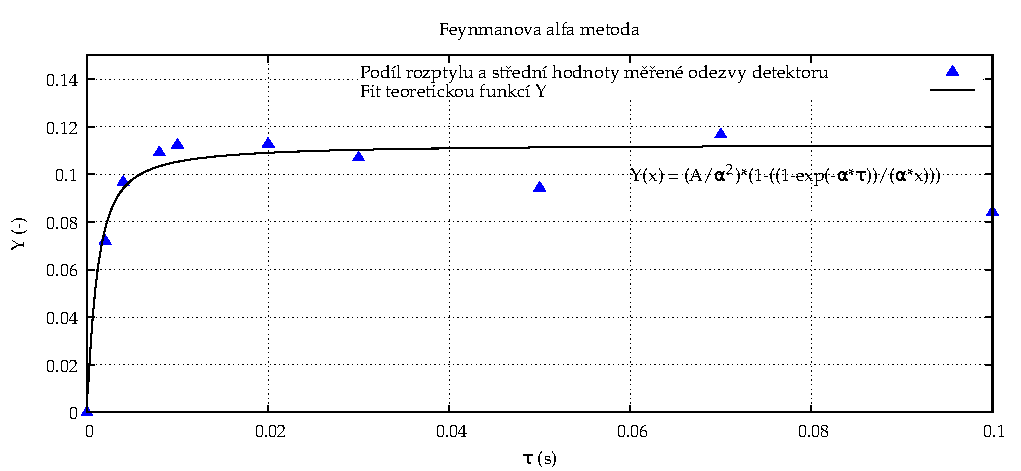
\includegraphics{img/graphy_feynman.pdf}
    \caption{Feynmanova-alfa metoda aplikovaná na podkritický soubor VR-2.}
    \label{fig:graph_feynman_alpha}
\end{figure}
\end{comment}

\subsection{Stanovení charakteristiky absorpční tyče}

\subsubsection{Absorpční tyč}

Absorpční tyče jsou důležitým nástrojem pro řízení reaktoru ve jaderné elektrárně. Jejich správná manipulace a kalibrace jsou nezbytné pro zajištění bezpečného provozu reaktoru.

Absorpční tyče jsou v jaderných reaktorech používány nejen jako regulační, ale i jako ochranné prvky. Absorpčním materiálem bývá velmi často bór (absorbuje $^{10}$B) ve formě karbidu boru B$_4$C nebo ocelových slitin obohacených borem, dále kadmium (VR-1), stříbro, indium nebo hafnium. 

Absorpční tyče, které plní ochranné funkce, jsou obvykle označovány jako \textbf{bezpečností tyče}. Jejich pozice v AZ je volena tak, aby byly schopny v krátkém časovém úseku vnést do reaktoru dostatečné množství záporné reaktivity, které bezpečně odstaví reaktor. 

Absorpční tyče, které plní funkci regulačního orgánu jsou označovány jako \textbf{regulační tyče} a slouží k dosahování kritického stavu reaktoru, uvádění reaktoru do podkritického nebo nadkritického stavu, zvyšování či snižování výkonu, kompenzaci krátkodobých, ale i dlouhodobých změn reaktivity. Na těchto tyčích je vázán kladný přebytek reaktivity (tzv. provozní přebytek reaktivity), který lze dle potřeby uvolnit.

Jelikož absorpční tyče plní v jaderném reaktoru jak bezpečnostní, tak i provozní roli, je nutné znát detailně jejich charakteristiky, které popisují vliv tyče na násobící schopnost reaktoru. Mezi základní charakteristiky absorpční tyče patří:

\begin{itemize}
    \item váha tyče -- $\rho_0$ (celková záporná reaktivita, která je na tyči vázaná),
    \item integrální charakteristika -- $\rho(\text{z})$ (závislost mezi změnou reaktivity a polohou),
    \item diferenciální charakteristika -- $\Delta\rho(\text{z})/\Delta z$ (derivace integrální charakteristiky, závislost mezi změnou reaktivity a změnou polohy).
\end{itemize}

K určování charakteristik absorpčních tyčí lze použít metody měření reaktivity, které byly prezentovány v předchozích kapitolách. 

%Charakteristikou absorpční tyče je míněn vliv tyče na násobící schopnost reaktoru v závislosti na její poloze nebo změně polohy v AZ, přičemž rozeznáváme integrální a diferenciální charakteristiku. Dalším důležitým parametrem, který je s tímto charakteristikami spojen, je váha absorpční tyče. Integrální charakteristika absorpční tyče představuje závislost reaktivity vnesené do AZ reaktoru na aktuální poloze tyče, tj. $ \rho(z) $. Diferenciální charakteristika absorpční tyče představuje závislost změny reaktivity na změně polohy absorpční tyče, tj. $ \Delta \rho(z)/\Delta z $. Váha tyče představuje reaktivitu, kterou je schopna do reaktoru vnést jako kompenzační nebo záporného vlastnosti, resp. jako změnu reaktivity v dané poloze reaktoru.

\subsubsection{Kalibrační křivka tyče vycházející z poruchové teorie}

Na základě poruchové teorie je možné odvodit teoretický stav pro integrální charakteristiku absorbční tyče jako:

\begin{equation*}
    \rho_\text{por} (z) = \rho_\text{0} \cdot \left(\frac{z}{H} - \frac{1}{2\pi}\cdot \sin\frac{2\pi z }{H} \right),
\end{equation*}

kde $\rho_\text{0}$ je váha tyče, $H$ je celková délka AZ a $z$ vzdálenost tyče od dolní koncové polohy. Diferenciální charakteristiku je možné získat její derivací.

Základní myšlenkou poruchové teorie je očekávání, že pokud se dostatečně málo změní fyzikální prostředí, v němž se nachází studovaný systém, potom se dostatečně málo změní i jeho vlastnosti a chování.

\subsubsection{Metoda inverzních četností}

Kalibrace absorpční tyče metodou inverzních četností je založena na násobení neutronů, které jsou \textbf{emitovány vnějším zdrojem neutronů v podkritickém systému}. Aktuální násobící schopnost, tedy míra podkritičnosti takovéhoto systému, je měněna absorpční tyčí, která je předmětem kalibrace. %Výsledkem kalibrace je pak integrální charakteristika neboli tzv. kalibrační křivka.

Předpokládejme, že máme zdroj neutronů umístěný v podkritickém reaktoru s $k_{ef} <$  1, který emituje konstantně $S_0$ neutronů. Pak lze celkový počet neutronů $N$, získaných jak ze zdroje, tak z násobení v AZ reaktoru, popsat následujícím vztahem:

\begin{equation*}
N = S_0 + S_0 \cdot k_{ef} + S_0 \cdot k_{ef}^2 + S_0 \cdot k_{ef}^3 + \ldots + S_0 \cdot k_{ef}^m,
\end{equation*}

což představuje součet členů geometrické posloupnosti s kvocientem $k_{ef}$. Vztah pro měřenou četnost $CR$ získáme součtem $m$ členů posloupnosti v rovnici výše a jeho vynásobením účinností detekčního systému $\varepsilon$:

\begin{equation*}
CR = \varepsilon \cdot S_0 \cdot \frac{1 - k_{ef}^m}{1 - k_{ef}},
\end{equation*}

kde $m$ je počet neutronových generací.

Je-li $ k_{ef} < 1 $ a $ m \rightarrow \infty $, pak lze rovnici zjednodušit na tvar:

\begin{equation*}
CR = \varepsilon \cdot S_0 \cdot \frac{1}{1 - k_{ef}}
\end{equation*}

a vyjádřit $ k_{ef} $ ve formě:

\begin{equation*}
k_{ef} = 1 - \frac{\varepsilon \cdot S_0}{CR}
\end{equation*}

Změnu reaktivity po vytažení tyče z dolní koncové polohy do polohy $ z $ je možné charakterizovat na základě Obrázku \ref{fig:charakteristikaTyče} následujícím vztahem:

\begin{equation*}
\Delta \rho(z) = \rho_0 \cdot \frac{ \rho(z) - \rho_\downarrow}{\rho_\uparrow - \rho_\downarrow},
\end{equation*}

kde:

\begin{itemize}%[noitemsep]
    \item $\rho_0$ je váha řídicí tyče,
    \item $\rho(z)$ je reaktivita v případě, že je kalibrovaná tyč v aktuální poloze $ z $,
    \item $\rho_\downarrow$ je reaktivita v případě, že je kalibrovaná tyč v dolní koncové poloze,% (0 mm pro reaktor VR-1),
    \item $\rho_\uparrow$ je reaktivita v případě, že je kalibrovaná tyč v horní koncové poloze.% (680 mm pro reaktor VR-1).
\end{itemize}

Vyjádříme-li reaktivitu pomocí koeficientu násobení: $\rho = \frac{(k_{ef} - 1)}{k_{ef}}$ a dosadíme do rovnice, můžeme tuto rovnici přepsat:

\begin{equation*}
\Delta \rho(z) = \rho_0 \cdot \frac{\frac{k_{ef}(z) - 1}{k_{ef}(z)} - \frac{k_{ef,\downarrow} - 1}{k_{ef,\downarrow}}}{\frac{k_{ef,\uparrow} - 1}{k_{ef,\uparrow}} - \frac{k_{ef,\downarrow} - 1}{k_{ef,\downarrow}}}
\end{equation*}

Dosadíme-li za $ k_{ef} $ vztah pro $k_{ef}$, pak rovnice přechází na tvar:

\begin{equation*}
\Delta \rho(z) = \rho_0 \cdot \frac{\frac{1}{CR(z)} - \frac{1}{CR_\downarrow}}{\frac{1}{CR_\uparrow} - \frac{1}{CR_\downarrow}} \cdot \dfrac{k_{ef, \uparrow}}{k_{ef}(z)},
\end{equation*}

a jelikož je $\dfrac{k_{ef, \uparrow}}{k_{ef}(z)} \approx 1$, můžeme tento podíl zanedbat a získat tak konečný vztah, který umožňuje kalibraci tyče metodou inverzní četnosti:

\begin{equation}
\boxed{\Delta \rho(z) = \rho_0 \cdot \frac{\frac{1}{CR(z)} - \frac{1}{CR_\downarrow}}{\frac{1}{CR_\uparrow} - \frac{1}{CR_\downarrow}}.}
\end{equation}

\begin{figure}[H]
    \centering
    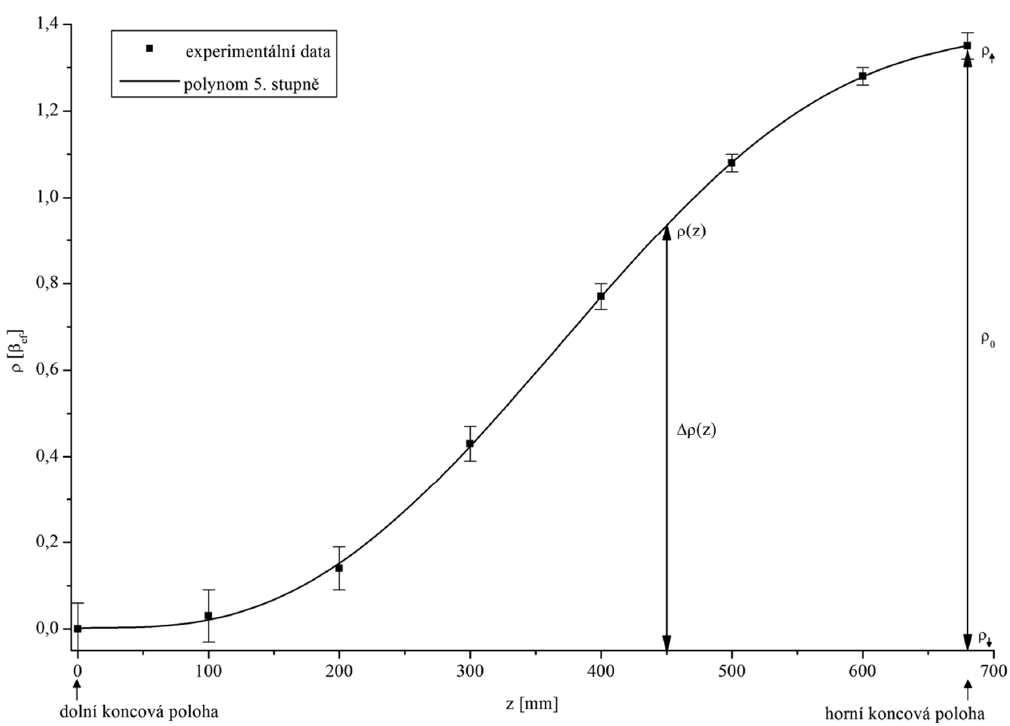
\includegraphics[scale=0.45]{img/CharakteristikaTyče.png}
    \caption{Integrální charakteristika tyče.}
    \label{fig:charakteristikaTyče}
\end{figure}

\subsubsection{Metoda s reaktimetrem}

K rychlé kalibraci absorpční tyče lze využít reaktimetr, který poskytuje informaci o časové závislosti podle vztahu:

\begin{equation} \label{rektimetr}
    \boxed{
    \begin{multlined}
    \rho_\text{kin} (t) = \frac{\Lambda \cdot \frac{dn(t)}{\text{d}t} + \beta_\text{ef}-n_\text{0}\cdot \sum_{i=1}^6\beta_{\text{ef},i}\cdot e^{-\lambda_i \cdot t}}{n(t)} -\\
    - \frac{\sum_{i=1}^6\beta_{\text{ef},i}\cdot \lambda_i \cdot \int_0^t n(t') \cdot e^{-\lambda_i \cdot t'} \text{d}t' -\Lambda \cdot S(t)}{n(t)}.
    \end{multlined}}
\end{equation}

Do reaktoru, resp. z reaktoru lze zavádět resp. vytahovat kalibrovanou absorpční tyč
známou konstantní rychlostí $v$, lze pak na základě dat z reaktimetru $\rho_\text{kin}$(t) a vztahu mezi
rychlostí pohybu tyče a její polohy ($z = v \cdot t$) získat závislost reaktivity na aktuální poloze tyče $\rho_\text{kin} (z)$, tedy integrální charakteristiku.